% Geometry, font
\documentclass[12pt, letter]{article}
\usepackage[margin=0.8in]{geometry}
\usepackage[T1]{fontenc}
\usepackage{fourier}
\usepackage{titling}
\setlength{\droptitle}{-5em} 
\usepackage[parfill]{parskip}
\usepackage{graphicx}
\graphicspath{{imgs/}}
\usepackage{hyperref}

% Math stuff
\usepackage{amssymb}
\usepackage{bm}

% Code Highlighting
\usepackage{minted}
\usemintedstyle{solarizedlight}

\author{Zach Neveu}
\title{ Day 17 Notes }

\begin{document}
\maketitle
\section{Agenda}%
\label{sec:agenda}

\begin{itemize}
	\item Quiz
	\item Review of Dynamic Programming
\end{itemize}

\section{Dynamic Programming}%
\label{sec:dynamic_programming}
\begin{itemize}
	\item Problem: order of matrix multiplication
	\item Key concepts
	\begin{itemize}
		\item All solutions must have a final multiplication
		\item Final multiplication cost is LHS+RHS+combining
		\item For optimal soln, LHS, RHS must each be optimal
		\item This is true recursively
	\end{itemize}
	\item Notation
	\begin{itemize}
		\item $m[i,j]$ - optimal sub-product cost $\prod_{k=i}^j A_k$
		\item $m[i,j] = 0$ if  $i==j$, else $argmin_k(m[i,k]+m[k+1,j]+p_{i-1}p_kp_j)$
	\end{itemize}
\end{itemize}

\begin{minted}{Python}
# Recursive Matrix Chain
# Computes m[i,j]
def RMC(p,i,j):
    if i == j:
        return 0
    else:
        m[i,j] = MAXINT
        for k in range(i,j-1):
            q = RMC(p,i,k)+RMC(p,k+1,j)+p[i-1]*p[k]*p[j]
            if q < m[i,j]:
                m[i,j] = q
    return m[i,j]
\end{minted}

\begin{figure}[h]
    \centering
    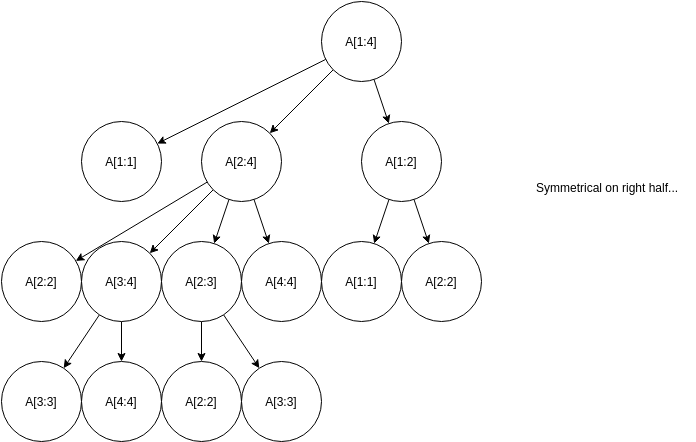
\includegraphics[width=0.8\textwidth]{rmc}
    \caption{Example RMC solution tree for $A_{1..4}$}
    \label{fig:rmc}
\end{figure}
\begin{itemize}
    \item Quiz question: modify this algorithm to keep track of best k at each step!
    \item Problem: Same sub-problems are solved over-and-over
    \item Just like recursive Fibonacci
    \item Solution: make $m[]$ global, and check if soln to subproblem has already been found. Use answer if it has.
    \item \textbf{memoization}: This process of saving already-computed solutions
\end{itemize}

\subsection*{Complexity}
\begin{itemize}
    \item $m$ matrix has $n^2$ entries
    \item Each entry computed exactly once
    \item Work to compute each entry (or at least one half (diagonal symmetry)):
    \begin{itemize}
        \item Each func call takes $O(n)$
        \item Total function takes $O(n*n^2) = O(n^{3})$
    \end{itemize}
\end{itemize}

\subsection*{Optimization}
\begin{itemize}
    \item Idea: instead of discovering tree recursively, why not just go through matrix in order and solve each subproblem?
    \item Organize as triangle (half matrix) w/ i,j along edges
    \item Build values from trivial diagonal to corner
    \item \textbf{dynamic programming} technically refers to this triangle approach, not the memoization
\end{itemize}

\subsection*{Dynamic TSP Example}
\begin{itemize}
    \item Is set of consecutive indices in HC also a HC? NO!
    \item Instead, given a subset of nodes, $s$, and some $k \in s$, $c(s,k)=$ min cost to start at node 1, visit all nodes in S, and end at k.
    \item $c ()$ can be expressed in terms of subproblems easily.
    \item Remove $k ^{th}$ node from the set and repeat with new $k$ 
    \item Try all $k$ and pick optimal
    \item Example
    \begin{itemize}
        \item c(\{2,4,6,7\}, 2) is min(c(\{4,6,7\},4)+w[4,2], c(\{4,6,7\}, 6)+w[6,2], \ldots)
        \item In general, $c(S,k) = min_{m\in S-\{k\}} c(s-\{k\},m)+w[m,k]$
    \end{itemize}
\end{itemize}


\end{document}
